%%%%%%%%%%%%%%%%%%%%%%%%%%%%%%%%%%%%%%%%%%%
%
% From a template maintained at https://github.com/jamesrobertlloyd/cbl-tikz-poster
%
% Code near the top should be fairly standard and not need to be changed
%  - except for the document class
% Code lower down is more likely to be customised
%
%%%%%%%%%%%%%%%%%%%%%%%%%%%%%%%%%%%%%%%%%%%

\pdfminorversion=4
\documentclass[portrait,a0b,final,a4resizeable]{include/a0poster}


\usepackage{multicol}
\usepackage{color}
\usepackage{morefloats}
\usepackage[pdftex]{graphicx}
\usepackage{rotating}
\usepackage{amsmath, amsthm, amssymb, bm}
\usepackage{array}
\usepackage{booktabs}
\usepackage{multirow}
\usepackage{hyperref}


\usepackage{include/picins}
\usepackage{tikz}
\usepackage{algorithm}% http://ctan.org/pkg/algorithms
\usepackage{algpseudocode}% http://ctan.org/pkg/algorithmicx
% \usepackage{algorithmic}
% \algsetup{linenosize=\small}
\usepackage{setspace}
\usepackage[hypcap=false,font=small,labelfont=bf]{caption} 
\usepackage{makecell}
\usetikzlibrary{shapes.geometric,arrows,chains,matrix,positioning,scopes,calc}
\tikzstyle{mybox} = [draw=white, rectangle]
\definecolor{darkblue}{rgb}{0,0.08,0.45}
\definecolor{blue}{rgb}{0,0,1}



\usepackage{nicefrac}
\newcommand{\vect}[1]{\underline{\smash{#1}}}
\renewcommand{\v}[1]{\vect{#1}}
\newcommand{\reals}{\mathds{R}}
\newcommand{\sX}{\mathcal{X}}
\newcommand{\sD}{\mathcal{D}}
\newcommand{\br}{}%{^{\text{\textnormal{ r}}}}
\newcommand{\cat}{^{\text{\textnormal{c}}}}

\usepackage{dsfont}
\usepackage{apacite}

\ProvidesPackage{preamble}

\usepackage{url}
\usepackage{array}
\usepackage{amsmath,amssymb,amsfonts,textcomp,amsthm}
\usepackage{booktabs}
\usepackage{relsize}
\usepackage{nicefrac}
\usepackage{graphicx}
\usepackage{rotating}
\usepackage{nth}
\usepackage{acronym}
\usepackage{bm}
%\usepackage{caption} \DeclareCaptionType{copyrightbox}
\usepackage{footnote}
\usepackage{color}

\usepackage{tabularx}
\newcolumntype{x}[1]{>{\centering\arraybackslash\hspace{0pt}}m{#1}}
\newcommand{\tabbox}[1]{#1}

\usepackage{hyperref}
\definecolor{mydarkblue}{rgb}{0,0.08,0.45}
\hypersetup{
    pdftitle={},
    pdfauthor={},
    pdfsubject={},
    pdfkeywords={},
    pdfborder=0 0 0,
    pdfpagemode=UseNone,
    colorlinks=true,
    linkcolor=mydarkblue,
    citecolor=mydarkblue,
    filecolor=mydarkblue,
    urlcolor=mydarkblue,
    pdfview=FitH}

\newcommand{\asdf}{$^{\textnormal{th}}$}

\newcommand{\binarysum}{\sum_{\bf{x} \in \{0,1\}^D}}
\newcommand{\expect}{\mathbb{E}}
\newcommand{\expectargs}[2]{\mathbb{E}_{#1} \left[ {#2} \right]}
\newcommand{\var}{\mathbb{V}}
\newcommand{\varianceargs}[2]{\mathbb{V}_{#1} \left[ {#2} \right]}
\newcommand{\variance}{\mathbb{V}}
\newcommand{\cov}{\operatorname{cov}}
\newcommand{\Cov}{\operatorname{Cov}}
\newcommand{\covarianceargs}[2]{\Cov_{#1} \left[ {#2} \right]}
\newcommand{\colvec}[2]{\left[ \begin{array}{c} {#1} \\ {#2} \end{array} \right]}
\newcommand{\tbtmat}[4]{\left[ \begin{array}{cc} {#1} & {#2} \\ {#3} & {#4} \end{array} \right]}

%\newcommand{\covskinny}[2]{\var\!\left(#1\middle\vert#2\right)} 

\newcommand{\acro}[1]{\textsc{#1}}
%\newcommand{\vect}[1]{\boldsymbol{#1}}
%\newcommand{\vect}[1]{{\bf{#1}}}
\newcommand{\mat}[1]{\mathbf{#1}}
\newcommand{\pderiv}[2]{\frac{\partial #1}{\partial #2}}
\newcommand{\npderiv}[2]{\nicefrac{\partial #1}{\partial #2}}

\newcommand{\pha}{^{\phantom{:}}}

\newcommand{\argmin}{\operatornamewithlimits{argmin}}
\newcommand{\argmax}{\operatornamewithlimits{argmax}}

% The following designed for probabilities with long arguments

\newcommand{\Prob}[2]{P\!\left(\,#1\;\middle\vert\;#2\,\right)}
\newcommand{\ProbF}[3]{P\!\left(\,#1\!=\!#2\;\middle\vert\;#3\,\right)}
\newcommand{\p}[2]{p\!\left(#1\middle\vert#2\right)}
\newcommand{\po}[1]{p\!\left(#1\right)}
\newcommand{\pF}[3]{p\!\left(\,#1\!=\!#2\;\middle\vert\;#3\,\right)} 
\newcommand{\mean}[2]{{m}\!\left(#1\middle\vert#2\right)}
%\newcommand{\novmean}[2]{{m}\!\left(#1\middle\vert#2\right)}
%\newcommand{\novcov}[2]{\var\!\left(#1\middle\vert#2\right)}
%\newcommand{\cov}[2]{\var\!\left(#1\middle\vert#2\right)} 
%\newcommand{\pskinny}[2]{p\!\left(#1\;\middle\vert\;#2\right)}
%\newcommand{\meanskinny}[2]{{m}\!\left(#1\middle\vert#2\right)}
%\newcommand{\covskinny}[2]{\var\!\left(#1\middle\vert#2\right)} 

\newcommand{\vI}{\mat{I}}
\newcommand{\vX}{\mat{X}}
\newcommand{\vY}{\mat{Y}}
\newcommand{\vZ}{\mat{Z}}
\newcommand{\vK}{\mat{K}}
\newcommand{\vs}{\vect{s}}
\newcommand{\va}{\vect{a}}
\newcommand{\vA}{\vect{A}}
\newcommand{\vb}{\vect{b}}
\newcommand{\vB}{\mat{B}}
\newcommand{\vR}{\mat{R}}
\newcommand{\vS}{\mat{S}}
\newcommand{\vu}{\vect{u}}
\newcommand{\vk}{\vect{k}}
\newcommand{\vc}{\vect{c}}
\newcommand{\vC}{\mat{C}}
\newcommand{\vw}{\vect{w}}
\newcommand{\vx}{\vect{x}}
\newcommand{\vy}{\vect{y}}
\newcommand{\vz}{\vect{z}}
\newcommand{\vmu}{\vect{\mu}}
\newcommand{\vpi}{\vect{\pi}}
\newcommand{\vphi}{\vect{\phi}}
\newcommand{\vSigma}{\mat{\Sigma}}
\newcommand{\vtheta}{\vect{\theta}}
\newcommand{\vl}{\vect{l}}
\newcommand{\vq}{\vect{q}}
\newcommand{\vf}{\vect{f}}
\newcommand{\vg}{\vect{g}}
\newcommand{\vell}{\vect{\ell}}
\newcommand{\ve}{\vect{\epsilon}}
\newcommand{\vzero}{\vect{0}}
\newcommand{\vone}{\vect{1}}

\newcommand{\He}{\mathcal{H}}
\newcommand{\normx}[2]{\left\|#1\right\|_{#2}}
\newcommand{\Hnorm}[1]{\normx{#1}{\He}}
\newcommand{\mmd}{{\rm MMD}}


\newcommand{\mf}{\bar{\vf}}

\newcommand{\st}{_\star}

\newcommand{\inv}{^{{\mathsmaller{-1}}}}
\newcommand{\tohalf}{^{{\mathsmaller{\nicefrac{1}{2}}}}}

\newcommand{\Normal}{\mathcal{N}}
\newcommand{\N}[3]{\mathcal{N}\!\left(#1|#2,#3\right)}
\newcommand{\Nt}[2]{\mathcal{N}\!\left(#1,#2\right)}
\newcommand{\bN}[3]{\mathcal{N}\big(#1|#2,#3\big)}
\newcommand{\boldN}[3]{\text{\textbf{\mathcal{N}}}\big(#1;#2,#3\big)}
\newcommand{\ones}[1]{\mat{1}_{#1}}
\newcommand{\eye}[1]{\mat{E}_{#1}}
\newcommand{\tra}{{^\ensuremath{\mathsf{T}}}}
\newcommand{\trace}{\operatorname{tr}}
\newcommand{\deq}{:=}
\newcommand{\degree}{^\circ}

\newcommand{\GPt}[2]{\mathcal{GP}\!\left(#1,#2\right)}

\DeclareMathOperator{\chol}{chol}
\DeclareMathOperator{\diag}{diag}

\newcommand{\gp}{{\acro{gp}}}
\newcommand{\gplvm}{{\acro{gp-lvm}}}
\newcommand{\bmc}{{\acro{bmc}}}
\newcommand{\bq}{{\acro{bq}}}
\newcommand{\sbq}{{\acro{sbq}}}

\newenvironment{narrow}[2]{%
  \begin{list}{}{%
  \setlength{\topsep}{0pt}%
  \setlength{\leftmargin}{#1}%
  \setlength{\rightmargin}{#2}%
  \setlength{\listparindent}{\parindent}%
  \setlength{\itemindent}{\parindent}%
  \setlength{\parsep}{\parskip}}%
\item[]}{\end{list}}



\newcommand{\dist}{\ \sim\ }
\def\given{\,|\,}

% Table stuff
\newcolumntype{C}[1]{>{\centering\let\newline\\\arraybackslash\hspace{0pt}}m{#1}}
\newcolumntype{L}[1]{>{\raggedright\let\newline\\\arraybackslash\hspace{0pt}}m{#1}}
\newcolumntype{R}[1]{>{\raggedleft\let\newline\\\arraybackslash\hspace{0pt}}m{#1}}


\def\ie{i.e.\ }
\def\eg{e.g.\ }
\def\iid{i.i.d.\ }
%\def\simiid{\sim_{\mbox{\tiny iid}}}
\def\simiid{\overset{\mbox{\tiny iid}}{\sim}}
\def\eqdist{\stackrel{\mbox{\tiny d}}{=}}
\newcommand{\distas}[1]{\mathbin{\overset{#1}{\kern\z@\sim}}}

\def\Reals{\mathbb{R}}

\def\Uniform{\mbox{\rm Uniform}}
\def\Bernoulli{\mbox{\rm Bernoulli}}
\def\GP{\mathcal{GP}}
\def\GPLVM{\mathcal{GP-LVM}}

% Kernel stuff

\def\inputVar{x}
\def\InputVar{X}
\def\InputSpace{\mathcal{X}}
\def\outputVar{y}
\def\OutputSpace{\mathcal{Y}}
\def\function{f}
\def\kernel{k}
\def\KernelMatrix{K}
\def\SumKernel{\sum}
\def\ProductKernel{\prod}
\def\expression{e}

\def\SE{\acro{SE}}
\def\Per{\acro{Per}}
\def\RQ{\acro{RQ}}
\def\Lin{\acro{Lin}}

\def\subexpr{{\cal S}}
\def\baseker{{\cal B}}
\def\numWinners{k}

\newcommand{\kSE}{{\acro{SE}}}
\newcommand{\kPer}{{\acro{Per}}}
\newcommand{\kLin}{{\acro{Lin}}}
\newcommand{\kRQ}{{\acro{RQ}}}


% Proof stuff
\theoremstyle{plain}
\newtheorem{theorem}{Theorem}[section]
\newtheorem{lemma}[theorem]{Lemma}
\newtheorem{prop}[theorem]{Proposition}
\newtheorem*{cor}{Corollary}


%%%%%%%%%%%%%%%%%%%%%%%%%%%%%%%%%%%%%%%%%%%
%
% myfig
%
% \myfig - replacement for \figure
% necessary, since in multicol-environment 
% \figure won't work        
%                 
%%%%%%%%%%%%%%%%%%%%%%%%%%%%%%%%%%%%%%%%%%%

\newcommand{\myfig}[3][0]{
\begin{center}
  \vspace{1.5cm}
  \includegraphics[width=#3\hsize,angle=#1]{#2}
  \nobreak\medskip
\end{center}}

%%%%%%%%%%%%%%%%%%%%%%%%%%%%%%%%%%%%%%%%%%%
%
% mycaption                
%
% \mycaption - replacement for \caption
% necessary, since in multicol-environment \figure and
% therefore \caption won't work
%
%%%%%%%%%%%%%%%%%%%%%%%%%%%%%%%%%%%%%%%%%%%

%\newcounter{figure}
\setcounter{figure}{1}
\newcommand{\mycaption}[1]{
  \vspace{0.5cm}
  \begin{quote}
    {{\sc Figure} \arabic{figure}: #1}
  \end{quote}
  \vspace{1cm}
  \stepcounter{figure}
}

%%%%%%%%%%%%%%%%%%%%%%%%%%%%%%%%%%%%%%%%%%%
%
% Some standard colours
%
%%%%%%%%%%%%%%%%%%%%%%%%%%%%%%%%%%%%%%%%%%%

\definecolor{camlightblue}{RGB}{0  , 47, 101}
\definecolor{camdarkblue}{rgb}{0, 0.203, 0.402}
\definecolor{camred}{rgb}{1, 0.203, 0}
\definecolor{camyellow}{rgb}{1, 0.8, 0}
\definecolor{lightblue}{rgb}{0, 0, 0.80}
\definecolor{white}{rgb}{1, 1, 1}
\definecolor{whiteblue}{rgb}{0.80, 0.80, 1}

%%%%%%%%%%%%%%%%%%%%%%%%%%%%%%%%%%%%%%%%%%%
%
% Some look and feel definitions
%
%%%%%%%%%%%%%%%%%%%%%%%%%%%%%%%%%%%%%%%%%%%

\setlength{\columnsep}{0.03\textwidth}
\setlength{\columnseprule}{0.0006\textwidth}
\setlength{\parindent}{0.0cm}

%%%%%%%%%%%%%%%%%%%%%%%%%%%%%%%%%%%%%%%%%%%
%
% \mysection - replacement for \section*
% 
% Puts a pretty box around some text
% TODO - any other thoughts for what this box should look like
%
%%%%%%%%%%%%%%%%%%%%%%%%%%%%%%%%%%%%%%%%%%%

\tikzstyle{mysection} = [rectangle, 
									draw=none, 
									shade, 
									outer color=camlightblue,
									inner color=camlightblue,
									text width=0.965\columnwidth,
									text centered,
									rounded corners=20pt,
									minimum height=0.09\columnwidth]

\newcommand{\mysection}[1]
{
\begin{center}
  \begin{tikzpicture}
    \node[mysection] {\color[rgb]{1,1,1}\sffamily\bfseries\LARGE#1};
  \end{tikzpicture}
\end{center}
}

%%%%%%%%%%%%%%%%%%%%%%%%%%%%%%%%%%%%%%%%%%%
%
% Set the font
%
% TODO - Not sure what a canonical choice is - feel free to modify
%
%%%%%%%%%%%%%%%%%%%%%%%%%%%%%%%%%%%%%%%%%%%

\renewcommand{\familydefault}{cmss}
\sffamily

%%%%%%%%%%%%%%%%%%%%%%%%%%%%%%%%%%%%%%%%%%%%%%%%%%%%
%%%               Background                     %%%
%%%%%%%%%%%%%%%%%%%%%%%%%%%%%%%%%%%%%%%%%%%%%%%%%%%%

\newcommand{\background}[3]{
  %\definecolor{cgradbegin}{#1}
  %\definecolor{cgradend}{#2}
 % \psframe[fillstyle=gradient,gradend=cgradend,
 % gradbegin=cgradbegin,gradmidpoint=#3](0.,0.)(1.\textwidth,-1.\textheight)
}




%%%%%%%%%%%%%%%%%%%%%%%%%%%%%%%%%%%%%%%%%%%%%%%%%%%%
%%%                pcolumn                       %%%
%%%%%%%%%%%%%%%%%%%%%%%%%%%%%%%%%%%%%%%%%%%%%%%%%%%%

\newenvironment{pcolumn}[1]{
  \begin{minipage}{#1\textwidth}
  \begin{center}
}{
  \end{center}
  \end{minipage}
}



%%%%%%%%%%%%%%%%%%%%%%%%%%%%%%%%%%%%%%%%%%%%%%%%%%%%
%%%                pbox                          %%%
%%%%%%%%%%%%%%%%%%%%%%%%%%%%%%%%%%%%%%%%%%%%%%%%%%%%

\definecolor{lcolor}{rgb}{0, 0, 0.80}
\definecolor{gcolor1}{rgb}{1, 1, 1}
\definecolor{gcolor2}{rgb}{.80, .80, 1}

  % \def\fc{fillcolor}
  % \def\getfc #1=#2\par{\def\ffc{#1} \ifx\ffc\fc #2\fi} 
  % \def\getfillcolor #1,#2\par{\getfc #1\par \getfc #2\par}

 %  \newcommand{\psshadowbox}[2]{%[2][magenta]{
%      \fbox{Input arg: #1}
%      \fbox{#1} 
%      \fbox {\getfillcolor #1\par}
%      \def\col{\getfillcolor #1\par}
 
%      \let\coll=\col
%       \coll
 %     \colorbox{\col}{#2}
%       \mbox
   %   \coloredshadowbox{black}{\coll}{#2}
%   }

\newcommand{\pbox}[4]{
%\psshadowbox[#3]{
%\fbox{
\mbox{
\begin{minipage}[t][#2][t]{#1}
#4
\end{minipage}
}%}
}

%%%%%%%%%%%%%%%%%%%%%%%%%%%%%%%%%%%%%%%%%%%
%
% Poster environment
%
% Centres everything and can be used to define the width of the content
%
%%%%%%%%%%%%%%%%%%%%%%%%%%%%%%%%%%%%%%%%%%%

\newenvironment{poster}{
  \begin{center}
  \begin{minipage}[c]{\textwidth}
}{
  \end{minipage}
  \end{center}
}

\def\newarrow{\mbox{\begin{tikzpicture}
             \useasboundingbox{(-3pt,-4.5pt) rectangle (19pt,1pt)};
             \draw[->] (0,-0.07)--(17pt,-0.07);\end{tikzpicture}}}




\newcommand\transpose{{\textrm{\tiny{\sf{T}}}}}
\newcommand{\note}[1]{}
\newcommand{\hlinespace}{~\vspace*{-0.15cm}~\\\hline\\\vspace*{0.15cm}}
\newcommand{\embeddingletter}{g}
\newcommand{\bo}{{\sc bo}}
%\newcommand{\gp}{{\sc gp}}
\newcommand{\agp}{Arc \gp}



\begin{document}
\begin{poster}

% Potentially add some space at the top of the poster
\vspace{0\baselineskip}



%%% Header
\begin{center}
\begin{pcolumn}{0.99}

\newcommand{\logowidth}{0.06\textwidth}  % width mauna decomp

\pbox{0.99\textwidth}{}{linewidth=2mm,framearc=0.3,linecolor=camdarkblue,fillstyle=gradient,gradangle=0,gradbegin=white,gradend=white,gradmidpoint=1.0,framesep=1em}{
%%% U Toronto Logo
\hspace{2.3cm}
\begin{minipage}[c][][b]{\logowidth}
%  \begin{center}
    \vspace{-.18in}
    
\includegraphics[width=7cm,trim=9em 0em 9em 0em, clip]{badges/toronto}
   	% \hspace{35cm}
     
\includegraphics[width=7cm]{badges/uot_text.png}
\end{minipage}
%
%%% Title
\hspace{-5.0cm}
\begin{minipage}[c][9cm][c]{0.94\textwidth}
  \begin{center}
    \vspace{1.5cm}
    {\sffamily \Huge \textbf{Fast Weights Using Improved Memory Consolidation Designs}}\\[7.5mm]
    {\huge\sffamily Bowen Xu$^1$, Jimmy Ba$^2$, Richard Zemel$^1$\\[7.5mm]
  	\Large\texttt{Department of Computer Science, University of Toronto$^1$} \\[5mm]
  	\Large\texttt{Department of Electrical \& Computer Engineering, University of Toronto$^2$}
    }
  \end{center}
\end{minipage}
}
\end{pcolumn}
\end{center}

\vspace*{2.5cm}

\large


%%%%%%%%%%%%%%%%%%%%%%%%%%%%%%%%%%%%%%%%%%%%%%%%%%%%%%%%%%%%%%%%%%%%%%
%%% Begin of Document
%%%%%%%%%%%%%%%%%%%%%%%%%%%%%%%%%%%%%%%%%%%%%%%%%%%%%%%%%%%%%%%%%%%%%%


%%% Begin of Multicols-Enviroment
\begin{multicols}{3}
% 
\mysection{Abstract}
%
% 
\vspace{0.2in}
% 
{
\Large\sffamily
Storing better quality and greater amount of memory has been a difficult challenge for deep learning.
While the current artificial neural networks excel at tasks such as regression and classification, they fail to perform equally well on representing variables and storing data over long time.
We introduce an enhanced fast weights model that includes robust memory consolidation designs into the existing memory transformation mechanisms.
We show that our model comes with no additional costs, converges faster, and out-performs the original fast weights model on the associative retrieval tasks.
}
\begin{quote}
\vspace{0.2in}
\textbf{Keywords:} 
Fast Weights; Memory Consolidation; Memory Transformation; Deep Learning; Associative Retrieval
\end{quote}

\vspace{0.5in}

\mysection{Background}
%
Recently, Benna and Fusi have demonstrated that the combination of a power-law memory decay with a fast new memory adaptability maximizes both the memory storage and lifetime (2016).
Their method treats each piece of memory as random and uncorrelated, and maximizes the signal to noise ratio (SNR) of all the stored memories \cite{pld}.
Since Benna and Fusi use a power-law decay function which has the form of \emph{$t^{-\gamma}$}, $\gamma > 0.5$ is required for the function to converge (2016).
In addition, Benna and Fusi also suggest fast adaptability for the memory system which implies that the learning rate for new information should be exactly $1.0$ (2016).
% 
\vspace{0.25in}
\begin{align}
    &w_a(t) \equiv \sum_{t^{'} < t} \Delta w_a(t') r(t-t')
    \label{eq:memory} \\
    &S_{t^{'}}(t) \equiv \frac{1}{N}\left<\sum_{a=1}^N w_a(t)\Delta w_a(t') \right>
    \label{eq:signal} \\
    &N^2_{t^{'}}(t) \equiv \left<\frac{1}{N^2}\left(\sum_{a=1}^N w_a(t)\Delta w_a(t') \right)^2 \right> - S^2_{t^{'}}(t)
    \label{eq:variance} \\
    &S / N(t - t') = \sqrt{\frac{N r^2(t - t')}{\sum_{t" < t, t" \neq t'} r^2(t- t")}}
    \label{eq:snr}\\
    &\sum_{t" < t, t" \neq t'} r^2(t- t") \approx \int_{1}^{\infty} r^2(t) dt 
    \label{eq:decay}
\end{align}
\vspace{0.25in}

Recent advances in deep learning \cite{dnc, fw} have also shown that the use of an external memory with the artificial neural networks can significantly improve their abilities to retain information.
Ba et.\ al.\ devise a bidirectional memory transformation system.
Knowledge is not only transferred from the fast weights to the memory cells of a Recurrent Neural Network (RNN) through its hidden vector update but also transitioned from the memory cells to the fast weights as it is updated using the latest hidden vector at each time step.
Also, a learning rate $\eta$ and a decay rate $\lambda$ are included to control how much the fast weights should store new knowledge versus how quickly it should forget previous knowledge.
%
\vspace{0.25in}
\begin{align}
    &A(t) = \lambda A(t-1) + \eta h(t) h(t)^T
    \label{eq:external_memory} \\
    &h_s(t+1) = f(LN(Wh(t) + Cx(t) + A(t)h_{s-1}(t+1)))
    \label{eq:hidden_update} \\
    &h(t+1) = h_s(t+1) \label{eq:hidden_assign}
\end{align}
\vspace{1cm}

\mysection{Our Contribution}
We incorporate memory consolidation designs from \cite{pld} to the fast weights model \cite{fw}.
We keep the fast weights setup and the weights transferring mechanism unchanged.
However, our fast weights uses a learning rate of $\eta$ $=1.0$ instead of $\eta$ $=0.5$.
We also substitute the original exponential decay function $\lambda$ $=0.95^t$ to the product of a power-law decay function $\prod_{t=\tau}^{t=1} t^{-0.5}$ where $\tau$ is the number of time steps elapsed since the initial storage of a specific memory. 
 

\newpage 
\mysection{Decay Functions Comparisons}
 \vspace{-0.05cm}

Figure below shows that the product of power-law decay functions decays much faster than the original exponential decay function. 
We believe that because new information is stored in a greater portion than before, the fast weights has to decay its existing memory quicker to prevent memory interference. 
This design also forces the RNN to learn patterns quicker from the fast weights since existing information is quickly removed.

\vspace{-0.5in}
\myfig{figures/decays}{1}
\vspace{-1.0in}
\mycaption{Decay Functions Comparisons}
\vspace{0.5in}
%\begin{align*}
 %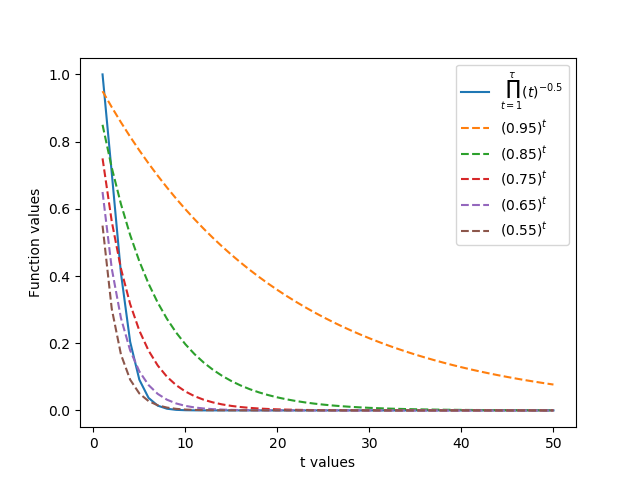
\includegraphics[width=\columnwidth,keepaspectratio=False]{figures/functions}
%\end{align*}

% 
\mysection{Experiments and Results}
We evaluate three RNN models on the associative retrieval tasks on three difficulty levels.
Our data consists of sequences of key-value pairs concatenated with two question marks and one query key.
The keys are lower case characters from the English alphabet chosen randomly without replacement, and the values are digits among 0 to 9 chosen randomly with replacement. \\

\begin{minipage}[c]{1\columnwidth}
        \centering
        \resizebox{!}{!}{
		\begin{tabular}{cc}
		Input String & \makecell{Target} \\
		\midrule
		c9k8j3f1??c & 9 \\
		\midrule
		j0a5s5z2??a & 5 \\
		\end{tabular}}
		\label{table:examples}
\end{minipage}
\vspace{0.25in}

Our training data contains $100,000$ sequences and our testing data contains $50,000$ sequences.
The difficulty levels are three key-value pairs (K = $3$), four key-value pairs (K = $4$), and twenty-six key-value pairs (K = $26$).
The following models are evaluated on correctly predicting the associated value of the query key: a vanilla RNN (CONTROL), the original fast weights model (RNN-LN-FW), and the improved fast weights model (RNN-LN-FW2).
All RNN models contain a single hidden layer with $50$ hidden units and are trained with $100$ iterations.\\

\mycaptiontable{Testing Accuracy of Different Models}
\begin{minipage}[c]{1\columnwidth}
        \centering
        \resizebox{!}{!}{
		\begin{tabular}{cccc}
		Model & \makecell{K = $3$} & \makecell{K = $4$} & \makecell{K = $26$} \\
		\midrule
		RNN-LN-FW2 & {$\bf 99.74\%$} & {$\bf 100\%$} & {$\bf 100\%$} \\
		\midrule
		RNN-LN-FW & $99.5\%$ & $99.71\%$ & $94.75\%$ \\
		\midrule
		\makecell{CONTROL} & $42.71\%$ & $34.49\%$ & $12.07\%$\\
		\end{tabular}}
		\label{table:compare_methods}
\end{minipage}

\vspace{-.25in}
\myfig{figures/k26}{1}
\vspace{-1.0in}
\mycaption{Testing Accuracy K = 26}

%\begin{align*}
%\hspace{-0.475in}
%  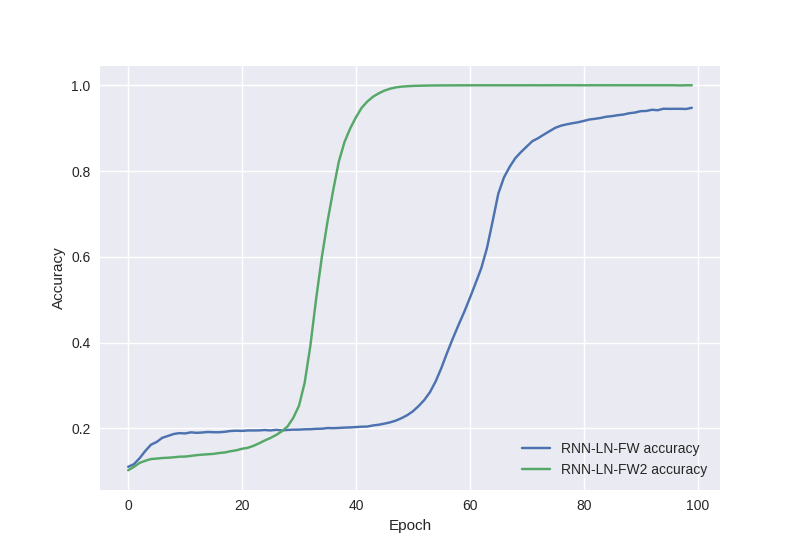
\includegraphics[width=30cm,keepaspectratio=False]{figures/k26}
%\end{align*}

\newpage
\mysection{Hidden Activations Visualization}
\vspace{-0.5cm}
\begin{align*}
\hspace{-0.475in}
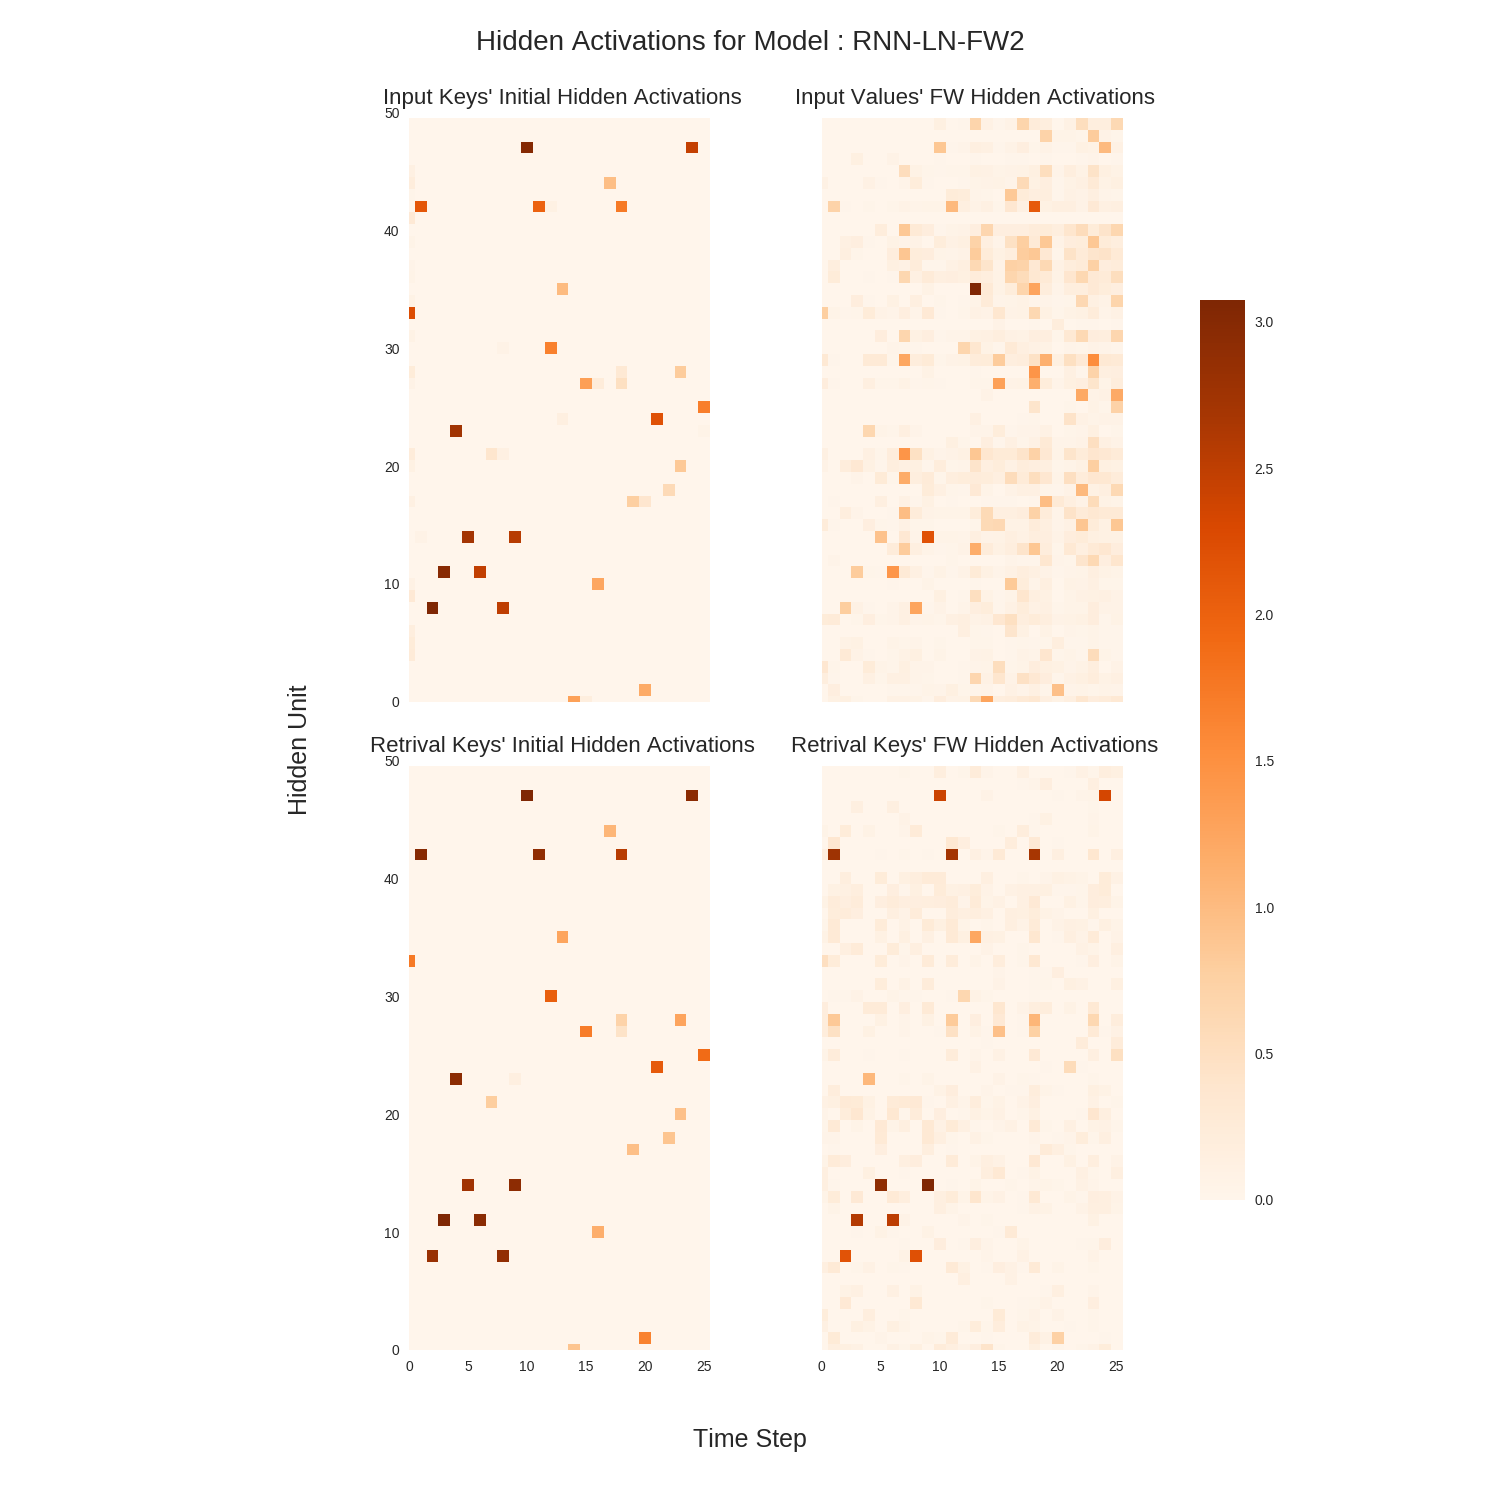
\includegraphics[width=30cm,keepaspectratio=False]{figures/Full_Comparison_RNN-LN-FW2_sample1}
\end{align*}
\vspace{-1.25in}
\mycaption{Hidden Activations for RNN-LN-FW2 K = 26}

\vspace{-.5in}
\begin{align*}
\hspace{-0.475in}
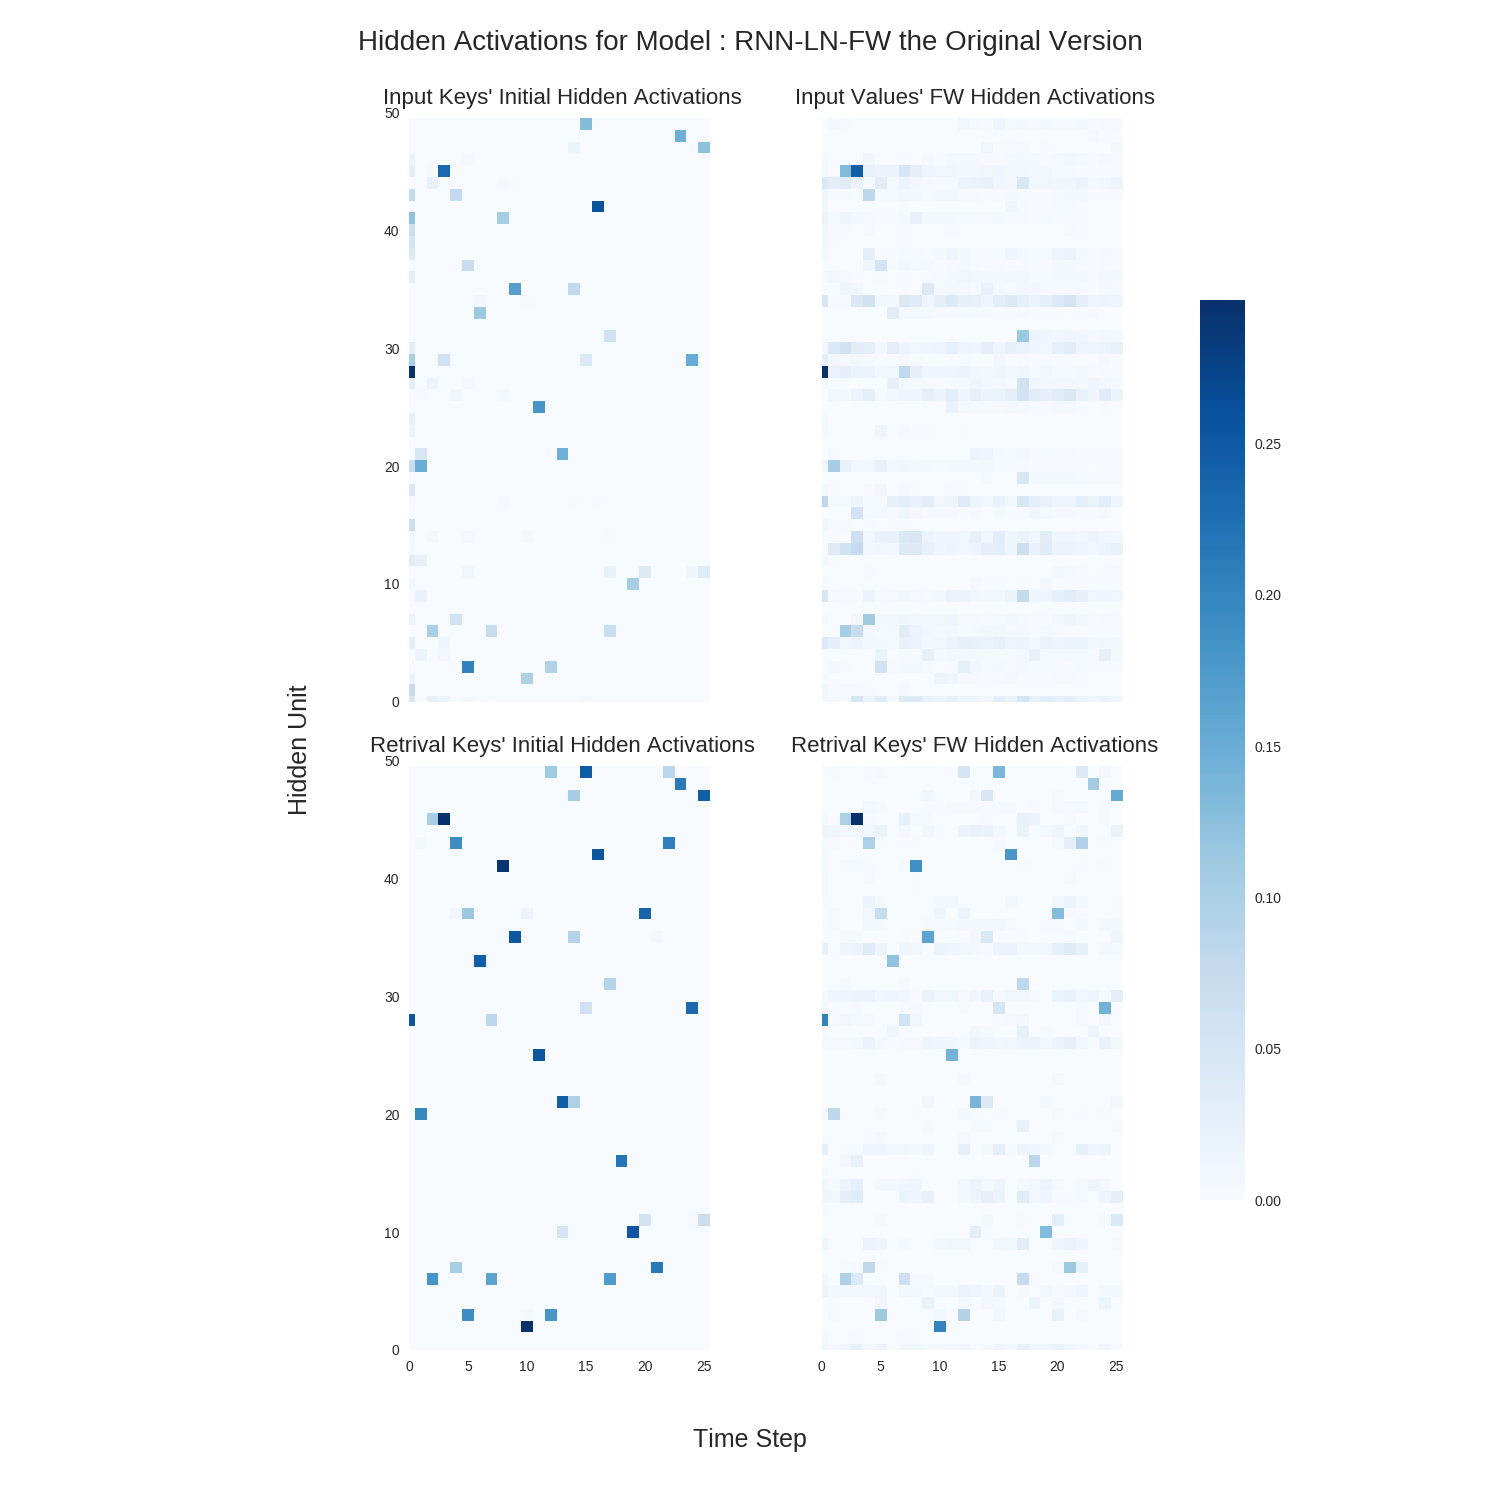
\includegraphics[width=30cm,keepaspectratio=False]{figures/Full_Comparison_RNN-LN-FW_sample3}
\end{align*}
\vspace{-1.25in}
\mycaption{Hidden Activations for RNN-LN-FW K = 26}

\vspace{1.cm}
\mysection{Conclusion and Future Work}
We introduce an enhanced fast weights model by incorporating memory consolidation designs from \cite{pld}.
We show that our model works better on the associative retrieval tasks and converges faster.
Our next direction is to evaluate the models on more difficult tasks such as sorting and repeated-copying.
We also intend to investigate other decay functions for the fast weights model.

\vspace{1.cm}

\mysection{References}
\small
\begingroup
\renewcommand{\section}[2]{}%
\bibliography{bib}
\endgroup
\bibliographystyle{apacite}

 
\end{multicols}
\end{poster}
\end{document}

